\documentclass[lettersize,journal]{IEEEtran}
\usepackage{amsmath,amsfonts}
\usepackage{algorithmic}
\usepackage{array}
\usepackage[caption=false,font=normalsize,labelfont=sf,textfont=sf]{subfig}
\usepackage{textcomp}
\usepackage{stfloats}
\usepackage{url}
\usepackage{verbatim}
\usepackage{graphicx}
\usepackage{balance}

\usepackage[UTF8]{ctex}


\begin{document}
\title{数据降维及可视化}
\author{姓名:尹伯豪\ 学号: 2112215089}

\maketitle

\begin{abstract}
This document describes the most common article elements and how to use the IEEEtran class with \LaTeX \ to produce files that are suitable for submission to the Institute of Electrical and Electronics Engineers (IEEE).  IEEEtran can produce conference, journal and technical note (correspondence) papers with a suitable choice of class options.
\end{abstract}

\section{The Design, Intent and \\ Limitations of the Templates}
\noindent The templates are intended to {\bf{approximate the final look and page length of the articles/papers}}. Therefore, {\bf{they are NOT intended to be the final produced work that is displayed in print or on IEEEXplore\textsuperscript{\textregistered}}}. They will help to give the authors an approximation of the number of pages that will be in the final version. The structure of the \LaTeX files, as designed, enable easy conversion to XML for the composition systems used by the IEEE's outsource vendors. The XML files are used to produce the final print/IEEEXplore\textsuperscript{\textregistered} pdf and then converted to HTML for IEEEXplore\textsuperscript{\textregistered}. Have you looked at your article/paper in the HTML version?

\section{\LaTeX \ Distributions: Where to Get Them}
\noindent IEEE recommends using the distribution from the \TeX User Group at \url{http://www.tug.org}. You can join TUG and obtain a DVD distribution or download for free  from the links provided on their website: \url{http://www.tug.org/texlive/}. The DVD includes distributions for Windows, Mac OS X and Linux operating systems.
 
\section{Where to get the IEEEtran Templates}
\noindent The {\bf{IEEE Template Selector}} will always have the most up-to-date versions of the \LaTeX\ and MSWord templates. Please see: \url{https://template-selector.ieee.org/} and follow the steps to find the correct template for your intended publication. Many publications use the IEEETran LaTeX templates, however, some publications have their own special templates. Many of these are  based on IEEEtran, but may have special instructions that vary slightly from those in this document.

\section{Document Class Options in IEEEtran}
\noindent At the beginning of your \LaTeX\ file you will need to establish what type of publication style you intend to use. The following list shows appropriate documentclass options for each of the types covered by IEEEtran.

There are other options available for each of these when submitting for peer review or other special requirements. IEEE recommends to compose your article in the base 2-column format to make sure all your equations, tables and graphics will fit the final 2-column format. Please refer to the document ``IEEEtran\_HOWTO.pdf'' for more information on settings for peer review submission if required by your EIC.

\section{How to Create Common Front Matter}
\noindent The following sections describe general coding for these common elements. Computer Society publications and Conferences may have their own special variations and will be noted below.
\subsection{Paper Title}
\noindent The title of your paper is coded as:

\begin{figure}[!t]
\centering
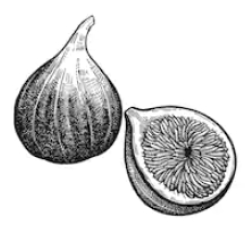
\includegraphics[width=2.5in]{fig1}
\caption{This is the caption for one fig.}
\label{fig1}
\end{figure}

\subsection{Paper Title}
\noindent The title of your paper is coded as:

\begin{thebibliography}{1}

\bibitem{ams}
{\it{Mathematics into Type}}, American Mathematical Society. Online available: 

\bibitem{oxford}
T.W. Chaundy, P.R. Barrett and C. Batey, {\it{The Printing of Mathematics}}, Oxford University Press. London, 1954.

\bibitem{lacomp}{\it{The \LaTeX Companion}}, by F. Mittelbach and M. Goossens

\bibitem{mmt}{\it{More Math into LaTeX}}, by G. Gr\"atzer

\bibitem{amstyle}{\it{AMS-StyleGuide-online.pdf,}} published by the American Mathematical Society

\bibitem{Sira3}
H. Sira-Ramirez. ``On the sliding mode control of nonlinear systems,'' \textit{Systems \& Control Letters}, vol. 19, pp. 303--312, 1992.

\bibitem{Levant}
A. Levant. ``Exact differentiation of signals with unbounded higher derivatives,''  in \textit{Proceedings of the 45th IEEE Conference on Decision and Control}, San Diego, California, USA, pp. 5585--5590, 2006.

\bibitem{Cedric}
M. Fliess, C. Join, and H. Sira-Ramirez. ``Non-linear estimation is easy,'' \textit{International Journal of Modelling, Identification and Control}, vol. 4, no. 1, pp. 12--27, 2008.

\bibitem{Ortega}
R. Ortega, A. Astolfi, G. Bastin, and H. Rodriguez. ``Stabilization of food-chain systems using a port-controlled Hamiltonian description,'' in \textit{Proceedings of the American Control Conference}, Chicago, Illinois, USA, pp. 2245--2249, 2000.

\end{thebibliography}

\end{document}


